%% Benjamin Williams <bwilliams@lincoln.ac.uk>
%% Get in touch if you have any questions or problems!
%% University of Lincoln Computer Science Thesis Template

%% @version     1.0.7
%% @lastchanged 26/04/2021

% The document class -- remove [harvard] if you want
% numeric-style referencing.
\documentclass[harvard]{lincolncsuthesis}
% Packages you want to use
% Packages you intend to use
% ..

% For example, if you want to render 
% the document in a different font you can
% use something like: 

%\usepackage{gentium}
%\usepackage{txfonts}
%\usepackage[sfdefault]{roboto}


% Or maybe you want clickable references in your thesis:
\usepackage{url}
\usepackage{float}
\usepackage{hyperref}
\hypersetup{%
    pdfborder = {0 0 0}
}
\usepackage[UKenglish]{babel}
\usepackage[T1]{fontenc}
\usepackage[utf8]{inputenc}
\usepackage{lmodern}
\usepackage{paralist}
\usepackage{fancyhdr}
\usepackage{amsmath, amssymb, amsfonts}
\usepackage{mathtools}
\usepackage{framed}
\usepackage{pstricks}
\usepackage{graphics}
\usepackage{nomencl}
\makenomenclature
\renewcommand{\nomname}{List of Abbreviations}

\usepackage[amsmath,framed, thmmarks, standard]{ntheorem}
\usepackage[usenames,dvipsnames,svgnames,table]{xcolor}
% \usepackage[backend=bibtex]{biblatex}
% \usepackage[backref=true, hyperref=true, firstinits=true, indexing=true, url=false, style=ieee, backend=biber,  doi=false, texencoding=utf8, bibencoding=utf8]{biblatex}

% Bibliography setup: import bib files
% Add in the .bib files you wish to add 
% into your document here. If you want to
% include others, just copy this line and
% change the path!

\addbibresource{./bib/references.bib}


% This thesis template also supports rendering
% a ludography. To cite games, make sure your reference
% in your bib file has keywords={game} in the bibtex item.
%
% See the bib file below for an example.

% \addbibresource{bib/ludography.bib}

% Your thesis details -- edit the file at the path below
% so it shows your name, title, etc. 
%% Below are a bunch of details for formatting your undergraduate thesis.
%% Make sure to fill each of these out.

% The title of your thesis (If your title is very large, consider prepending
% it with the \Large command
\title{\bfseries Brain-Computer Interface controlled simulated car using CARLA}

% Your name, as an author
\author{Mangal Deep B.M.}

% The degree
\thesisDegree{Master of  Engineering}

% The programme
\thesisProgramme{Embedded Systems for Mechatronics}

% The school name
\thesisSchool{Faculty of Information Technology}

% The university you're studying at (Lincoln!)
% The university (UoL)
\thesisUniversity{Dortmund University of Applied Sciences and Arts}

% Your student number
\thesisStudentNumber{7206937}
\thesisSupervisor{Dr. Andreas Becker}
% The date (which is shown last, you can just put a year in here):

\date{14-March-2023}



% What will be displayed in the header: the assessment item
\thesisHeaderContents{Master Thesis}

% Uncommenting the \thesisTurnOffHF line below will remove your name + id from the footer
% as well as removing the header contents. It is NOT recommended to do this
% as the presentation policy for assessed work in the SoCS requires
% these both of these. However, you may want to uncomment this for other
% reasons: i.e. when printing a personal copy which is NOT going to be
% submitted.
% -----
% \thesisTurnOffHF
% -----
% Not from the University of Lincoln? These commands below might
% be useful to you! Just uncomment them:
% ----------
% \thesisLogoPath{img/your_logo} 
% \thesisProgramme{Biology}
% \thesisSchool{School of Biology}
% \thesisCollege{College of Science}
% \thesisUniversity{Hogwarts School of Witchcraft and Wizardry}
% \thesisSubmissionText{This is some text}
% ----------


% Don't like the table of contents, list of figures, or list
% of tables? Do you want to disable them? If so, uncomment
% the appropriate lines below:
% ---------------
% \turnOffTOF          % List/Table of Figures
% \turnOffTOT          % List/Table of Tables
% \turnOffTOC          % Table of contents
% ---------------



% Do you want to enable listing sections before the thesis
% body in the table of contents? e.g. Abstract, List of Tables,
% List of Figures, etc.
% 
% This is what the command below does.
% 
% Just uncomment it if you this is what you desire:
% -----------------
% \enableManualTOCEntries

% But what if you want to remove "List of Figures", "List of Tables",
% and "Table of Contents" from the table of contents, but leave
% your original sections? That's ok, just uncomment the line below:
% ------------------
% \disableTableTOCEntries

\begin{document}

% First, make the title
\maketitle

% Input anything that can go before the acknowledgements 
%% The blank page environment allows you to insert
% pages into your thesis for specific things

\begin{blankpage}
    \chapterTitle{A blank page}
    This is an optional page environment you could use for things like:
	\begin{itemize}
		\item Your own custom preamble chapters (use \texttt{\textbackslash chapterTitle} for titles!)
		\item \emph{``This work is dedicated to Dad and Mom''}
		\item A copyright notice
		\item Additional notes
		\item Quotes
		\item List of publications
		\item An actual blank page
		\item Nomenclature / glossaries, etc.
	\end{itemize}
	It is not recommended to use this in your undergraduate thesis for submission. It has been left in here to make you aware of its existence. This is largely because it does not follow the guidelines set out for undergraduate theses, but you could include this environment for your own personal printed copy. Consult with your supervisor to see if you can use it. 
	
	In addition, you can pass an optional parameter to this environment with the value \texttt{c} to centre this text vertically on the page (use the \texttt{center} environment to align horizontally).
\end{blankpage}


% Then the abstract
\begin{abstract}
    This is where your abstract will go. Usually this is written last, after writing the entirety of your thesis.
\end{abstract}

% Then the acknowledgements
\begin{acknowledgements}
Firstly, I want to thank Dad and Mom.\footnote{Here is a footnote} Here is another note.
\end{acknowledgements}

% Print out the table of tables and table of figures and
% tell the template we're about to start the body of the
% thesis.
\thesisTables
% Indexes, Glossaries

\thesisBodyStart
% start of thesis body
% ---------------------------

% Include introduction
\chapter{Introduction}
% \section*{Introduction}
Human computer interaction has been evolving over the past decades. With development in technologies, the physical contact between the computer and the human is decreasing rapidly. Advanced systems which work on speech and gesture control still require a minimal effort from the user to interact with the machine. Though these effort seem to be mere, it is a challenging task for humans with disabilities. Systems which work on facial gestures bridge this gap to an extent but it does not completely decode the actual intent of the person. Brain Computer Interface paves way to encode the persons intent and thoughts without the need for any physical effort. It provides enormous capabilities for physically challenged people to express themselves just by their thoughts. 

Autonomous vehicles are the future of mobility, several companies around the world invest and research on new technologies to solve new challenges that appear in developing level 5 autonomy. The level of human interaction with the vehicle has been decreasing with increasing safety. However including humans in the loop is necessary at certain times to avoid any undesirable events. Level 5 autonomous vehicles is still a long way to go, but by bringing in a minimal interaction of the driver with the system, safety can be improved. One of the ways of achieving it is interfacing the thought and decision process of the driver to the autonomous vehicle, a process commonly referred to as Brain-Computer-Interface (BCI)\nomenclature{BCI}{Brain-Computer-Interface}. 

Once shown in science fiction novels and movies, Brain-Computer Interface (BCI) has become widely researched and developed in the academic institutions and industries in the past decades. It has been applied and tested on mammals for a wide range of applications. However it has its own challenges and limitations. With evolving technologies, new innovations and discoveries, BCI systems are built to understand and decode the brain waves better. The analysis of the brain signals have seen a shift in the paradigm with the introduction of machine learning techniques. 

Modern BCI design involves understanding brain dynamics, pattern recognition in the brain waves, deriving relevant features from the measured brain waves. However it is very challenging to create a BCI system that can work on any person, as the brain signals are task-specific and brain signal signatures are very unique to a person. The cortex folding and the relevant functional maps are different across individuals. Even for the very same person, the brain dynamics are non-stationary at all time scales. In addition, it is almost impossible to place the electrodes exactly on the same location for every recording sessions. Further the psychological states of the user such as boredom, distraction and similar factors play a significant role in the quality of the signal measured. The Signal-to-Noise Ratio (SNR) \nomenclature{SNR}{Signal-to-Noise Ratio} in a brain signal is very poor, making it difficult to obtain required information from brain signals. It is harder to spatially measure the data from one region as large collections of neurons are involved in many different activity, not just one. These challenges can vary a lot depending on the methods used to record and analyse the brain signals as well as the task that needs to be achieved. 

Given the challenges, the goal of this work is to steer a simulated car in the CARLA environment using brain signals obtained from the OpenBCI headgear. CARLA is an open-source simulator to develop, train and validate autonomous driving systems. OpenBCI is an open-source BCI platform that develops hardware and software for BCI scientific research. The brain signal from a 16 channel OpenBCI headgear is fed through a signal processing pipeline to extract the relevant Motor Imagery (MI) \nomenclature{MI}{Motor Imagery}features and classify the users intention. The signal preprocessing pipeline constitutes reliable and conventional signal processing techniques as well as state-of-the-art deep learning techniques. Several tools, libraries and frameworks such as MNE, Numpy, Scipy, Scikit-learn and PyTorch are used to achieve the goal. The communication between the OpenBCI system and the signal processing pipeline is established using Lab Streaming Layer (LSL)\nomenclature{LSL}{Lab Streaming Layer}. The signal processing pipeline classifies the signal into left, right or straight steering command and it is sent to CARLA through Robotic Operating System (ROS 1) framework\nomenclature{ROS 1}{Robotic Operating System-1}. The algorithms are packed into a ROS package which consists of multi-threaded nodes enabling real-time information transfer to CARLA. All the relevant code and references are made available in GitHub\cite{BCI_MotionControl}. Several open-source datasets are used to setup the basic brain signal processing pipeline and later tuned to work with the data obtained form the OpenBCI headgear.

\section{Environment setup}
The specifications of the system used for this project are listed in the table \ref{tb:specs}. The overview of the implemented system is given in the figure \ref{fig:MT_Overall}.

\begin{figure}[H] 
    \begin{center}
    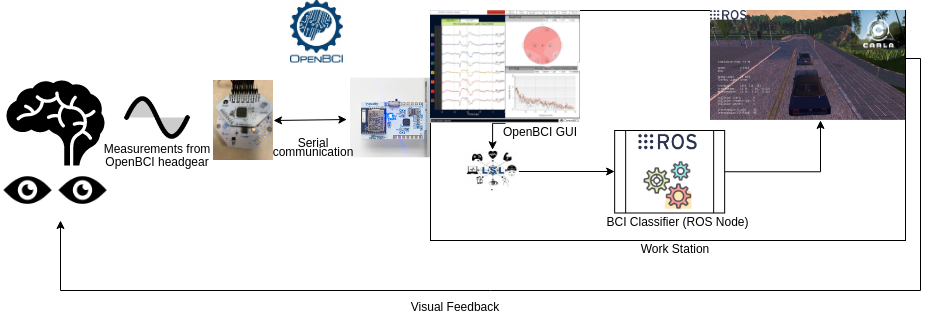
\includegraphics[width=1.0\textwidth]{images/MT_Overall.png}
    \caption{System overview}
    \label{fig:MT_Overall}
\end{center}
\end{figure}

\begin{table}[h!]
\centering
\arrayrulecolor[rgb]{0.8,0.8,0.8}
\begin{tabular}{|l|l|} 
\arrayrulecolor{black}\hline
\multicolumn{2}{|c!{\color{black}\vrule}}{Hardware Specifications}                                                                 \\ 
\hline
Processor                                   & AMD® Ryzen 7 4800h with radeon graphics × 16                                         \\ 
\arrayrulecolor[rgb]{0.8,0.8,0.8}\hline
RAM                                         & 16GB                                                                                 \\ 
\hline
Operating System                            & Ubuntu 20.04.5 LTS 64-bit                                                            \\ 
\hline
\# CPU cores                                & 8                                                                                    \\ 
\hline
GPU                                         & NVIDIA GeForce RTX 2060/ \\ 
                                            & RENOIR (renoir, LLVM 14.0.5, DRM 3.42, 5.15.0-56-generic)  \\ 
\hline
Graphic Card Driver                         & 515.86.01                                                                            \\ 
\hline
CUDA                                        & 11.6                                                                                 \\ 
\hline
cuDNN                                       & 8.3.2                                                                                \\ 
\hline
Cython + Daisy                              & 3.0.0                                                                                \\ 
\hline\\
\hline
%\multicolumn{1}{|l!{\color{black}\vrule}}{} & \multicolumn{1}{l!{\color{black}\vrule}}{}                                           \\ 
\arrayrulecolor{black}\hline
\multicolumn{2}{|c!{\color{black}\vrule}}{Software Specifications}                                                                 \\ 
\hline
Visual Studio Code                          & 1.74.0                                                                               \\ 
\arrayrulecolor[rgb]{0.8,0.8,0.8}\hline
OpenGUI                                     & 5.1.0                                                                                \\ 
\hline
CARLA                                       & 0.9.11 (py3.7-linux-x86\_64)                                                         \\ 
\hline\\
\hline
%\multicolumn{1}{|l!{\color{black}\vrule}}{} & \multicolumn{1}{l!{\color{black}\vrule}}{}                                           \\ 
\arrayrulecolor{black}\hline
\multicolumn{2}{|c!{\color{black}\vrule}}{Libraries and Frameworks}                                                                \\ 
\hline
Numpy                                       & 1.22.3                                                                               \\ 
\arrayrulecolor[rgb]{0.8,0.8,0.8}\hline
Pytorch                                     & 1.12.0+cu116                                                                         \\ 
\hline
MNE                                         & 1.2.0                                                                                \\ 
\hline
OpenCV                                      & 3.4.15                                                                               \\ 
\hline
scipy                                       & 1.8.1                                                                                \\ 
\hline
sklearn                                     & 1.1.1                                                                                \\ 
\hline
matplotlib                                  & 3.4.2                                                                                \\ 
\hline
kymatio                                     & 0.2.1                                                                                \\ 
\hline
PIL                                         & 7.0.0                                                                                \\ 
\hline
pandas                                      & 1.1.4                                                                                \\ 
\hline
Optuna                                      & 3.0.0                                                                                \\
\hline
\end{tabular}
\caption{\label{tb:specs} System and software specifications used for this project.}
\arrayrulecolor{black}
\end{table}

\section{Outline} 
The thesis is organized as follows the chapter \ref{ch:background} provides insight on different brain signal recording techniques, various EEG paradigms, brain signal extraction methods, artifact removal techniques used in this work and brief description of feature extraction, selection and classification steps, \ref{ch:sp_bci} discusses on various feature extraction and classification techniques used in brain signal analysis, \ref{ch:DL_bci} discusses on different SOTA Deep Learning techniques used in BCI signal analysis that can work as feature extractor and classifier. In chapter \ref{ch:cmp_bnch}, the tools and libraries used in this work are explained. The implemented algorithms are compared and analysed for different combinations. Finally chapter \ref{ch:ch_cncl} discusses about the challenges faced, further enhancements and the systems applicability for different use cases.

The following chapters provide deeper intuition and understanding of the methods researched and used in accomplishing this work. Finally the chosen algorithm is used to steer the simulated car in CARLA through ROS.

% Literature review / Background / Related work
% \chapter{Literature review}
% %%%%%%%%%%%%%%%%%%%%%%%%%%%%%%%%%%%%%%%%%%%%%%%%%%%%%%%%%%%%%%%%%%%%%%%%%%%%%%%%%%%%%%%%%%%%%%%
% Another cool thing about \LaTeX~is its referencing system. This template is set up to use harvard-style referencing. You can do this by using \texttt{\textbackslash citep\{citekey\}}. It will print out something like this: \citep{aad2012observation}. Or alternatively, you can use \texttt{\textbackslash cite\{citekey\}} to cite things like this: \cite{chatrchyan2012observation}. This template uses Bib\LaTeX~for referencing, with a Biber backend. This is primarily due to the extensive features Bib\LaTeX~provides, along with the option of glossaries. If you want to customise the referencing style, you can either modify the template slightly to use different options, or use \texttt{\textbackslash usepackage} again to reimport it. There's probably some commands to change its options after its been imported too.

% \section{Ludography}
% This thesis template also contains an optional ludography. This is primarily for Games Development students, who wish to cite games in their thesis. To use this, just put references into your bib file as usual with the game's details. Then, make sure \texttt{keywords} is set to \texttt{\{game\}}. This is what is used to determine which references are games, and which are actual papers. For a more elaborate example, see \texttt{bib/ludography.bib}.

% Also, make sure that the \texttt{title} key is actually the author of the game, and the \texttt{author} is the title of the game. The reason this is swapped around is because Bib\LaTeX~likes to print references out with the author first. Then, just add \texttt{\textbackslash printLudography} with an optional title argument to print out all citations like \texttt{\textbackslash printLudography} or \texttt{\textbackslash printLudography[Games]}.

% You can also use the \texttt{ludography} environment if you wish to print out some text before the list of games is printed. An example of this can be seen in \texttt{main.tex}. To cite games, you can \texttt{\textbackslash cite} it like any other reference. However, if you want it to display the title instead of the standard referencing style, you can use \texttt{\textbackslash citeGame} instead.

% Here is an example of a cited game with a normal reference style: ~\cite{spaceinvaders}. Ugh, pretty ugly. Instead, here the two are  cited in the next sentence as games with \texttt{\textbackslash citeGame}. Both \citeGame{spaceinvaders} and \citeGame{breakout} were games made by Atari. Much better!

% BCI Foundation
\chapter{Formulation}
\section*{Introduction}
    The goal of this work is to control the simulated car in CARLA using motor intent from the users brain activity. Motor Imagery is the information that needs to be extracted from the EEG data. There are several other information that can be  obtained and are broadly classified into Spontaneous EEG and Evoked Potential which are briefly explained.

\section{Brain Signal Acquisition/ Extraction}
Neurons are the basic computational unit of the nervous system. The electric signal recorder as brain wave is the result of electrochemical interations that occur at the outer membrane of neurons. In case of a event, the raises and falls of potential at the membrane of the neuron is called as action potential. The electrical activity at the neurons enable us to record and decode the brain activities. There are many ways to record the electrical activity and are broadly classified into invasive and non-invasive recording. Some technologies can also be used to stimulate neurons or brain regions, that allows BCIs to send feedback to brain based on interactions with the world. This work is only on Electroencephalography, a  noninvasive approach, hence the topic on invasive approaches and other noninvasive approaches are just briefly touched.

    \subsection{Invasive Approaches}
Approaches requiring some surgery where an electrode is placed in direct contact with required region in the brain are invasive methods of recording brain signals. These approaches are typically performed on animals such as monkeys, rats. In case of humans these approaches are carried on under strict clinical settings. As the recording sensor is in direct contact with the brain tissues, these provide higher quality signals with high SNR, higher spatial resolution and less spatial smearing compared to the noninvasive approaches.

    \subsubsection{Electrocorticography (ECoG)}
    ECoG is an extracortical invasive electrophysiological monitoring method \cite{2021}. Typically performed in a clinical setting, a strip of electrodes are placed on the surface of intrest on the brain. It has many advantages compared to other invasive approaches.

    \subsection{Noninvasive Approaches}
Approaches that gather brain signals over the surface of the scalp, without any surgery or electrodes being inserted into the skull are termed noninvasive approaches. The signals could be collected by measuring the electrical or the magnetic activity on the surface of the scalp. Some of the common noninvasive approaches are Electroencephalography (EEG), functional magnetic resonance imaging (fMRI), functional near-infrared spectroscopy (fNIRS), magnetoencephalography (MEG), and electrooculography (EOG).
    
%     \subsubsection{Functional Near-infrared Spectroscopy (fNIRS)}
% fNIRS uses near-infrared light to measure the degree of oxygenated and deoxygenated haemoglobin. The relative levels 

    \subsubsection{Electroencephalography (EEG)}
EEG is the most commonly used noninvasive approach used to measure brain electrical activity on the surface of the scalp. The electrodes are usually placed according to internationally recognized 10-20 system \cite{}. The spatial resolution of the signals depend on the number of electrodes used. The temporal resolution depends on how many samples the system could measure in a second. However the temporal resolution of the EEG signals is much better than the spatial resolution. In Comparison to invasive approaches, the EEG systems have poor spatial and temporal resolution, and very poor SNR. Since the measurement is taken
over the surface of the scalp, the obstruction of the skull and other tisses between cortex and the scalp act as a huge conductive surface leading to spatial smearing. In comparison to other noninvasive approaches EEGs have higher temporal resolution, tolerant to noise and artifacts, low cost and no exposure to high intensity magnetic fields.

    Spatial smearing is the effect by which all the electrodes tend to measure the same signal because of the conductive effect of the tissues between the cortex and scalp. It also very succeptible to other noises such as power-line, changind electrode impedance, eye movements, eye blinks, facial muscle movements and head movement. The brain signals measured from the EEG systems can be seperated into frequency bands, where each frequency band represents to a specific brain state
and level of awareness. The recorded brain signals contains information on various physiological, psychological, mental, sensory and cognitive activities. Hence it is required to analyse and extract the relevant information from the signal.

\section{EEG Paradigms}

\subsection{Spontaneous EEG}
Spontaneous EEG also referred as Oscillatory Activity includes a wide range of task typically without any external stimulation such as mental task, motor imagery,sleeping, under fatigue stage. BCI systems that work with spontaneous EEGs are also called Active BCI as they reuire conciously controlled thought independent from external events.BCI systems that work with spontaneous EEG are hard to train given their low SNR and variation in subjects.

    \subsubsection{Motor Imagery (MI)}
Imagining a motor movement without performing an actual movement is termed Motor Imagery. It is one of the widely researched EEG paradigm that is used in several applications where the user is limited in their motor movement capabilities. It also helps in mental rehersals as the person experience themselves performing the action. MI is due to two basic phenomena that occur in the brain onset of imagination - Event Related Desynchronization (ERD) and Event Related Synchronization (ERS). ERD/ERS refers to 
phenomena that the magnitude and the frequency distribution of the EEG signal power changes during a specific brain state. It is mostly observed in sensory, cognitive and motor tasks. During motor imagery contralateral ERD is observed in the mu band and after motor imagery ERS is observed in beta band.

Event Related Desynchronization (ERD) is due to activity of small set of neurons. A visual stimulation results in a short lasting attenuation or blocking of rhythm in the alpha band leading to power decrease of ongoing EEG signals. This decrease in the oscillatory is related to internally or externally paced events.

Event Related Synchronization (ERS) is due to activity of large set of neurons. The increase in oscillatory activity is again related to internally or externally paced events.It is characterized by short lasting amplitude enchancement.

\subsection{Evoked Potential (EP)}
Processing of physcal stimulus rather than higher processes that might involve memory and attention. BCI systems that work with EPs could be also called Reactive BCI as they rely on response to the stimulus provided. Few of the commonly researched EPs are described below.

    \subsubsection{Event Related Potential (ERP)}
It is the most widely researched EPs and it is further classified based on the stimulus used to trigger the brain waves: visual evoked potential when stimulated visually, audiotory evoked potential when stimulated with sound and somatosensory evoked potential when evoked with smell. The stimulus could be internal or external based on the BCI system. P300 is an important component in ERP and it is been widely used in many BCI systems exiisting in the marker. It refer to the postive peak that appears 300ms after the onset of stimulus.

    \subsubsection{Error Related Potential (ErRP)}
It is a result oof an errorous event. It is generated by the error processing mechanism in the human brain. It provides a feature rich feedback to the BCI system and helps to tune the sytem in the desirable way.

\section{Brain Signal Processing Pipeline}
The brain signal is fed through several signal processing algorithms to extract the best possible information. These processing algorithms are specifically chosen to  extract motor imagery data. The overall processing pipeline is given in the figure \ref{}. THe first few steps in the processing pipeline is the same for both conventional and deep learning approaches.  The variation is observed only at feature extraction and classification. These steps involved in the pipeline are explained in detail in the following sections.

\subsection{Data Extraction}
The input to the pipeline could be an online/offline data from OpenBCI headgear or publicly available open-source datasets. The open-source datasets were used in order to design the pipeline and later the pipeline is calibrated to work with data from OpenBCI headgear.

\subsubsection{OpenBCI headgear}
Before the experiment could be started several parameters are checked. In order to ensure the contact of electrodes on the users scalp, the impedance at the electrodes are monitored and adjusted untill they fall into acceptable threshold i.e. less than $750K\Omega$. Next the frequency filters are configured to avoid DC offset and electric powerline noises. However this filter is applied only to the visualizer and not to the recorded data. The electrodes are very succeptible to noises that appear around 25Hz even after
filtering the DC offset and powerline noises. Hence while performing the experiment the user is away from any electronic device.

Establihing a proper experiment is a key step in training the classifiers, By \cite{} each trail is recorded for 12 seconds, the setup used to gather data for a three class system that consists of a window sperated by a vertical line and two squares - yellow and blue,  in the centre initially. The beginning of each trial is marked by change in color of the vertical line then the subject is requested to be in a idle state for the first 5 seconds. The motor imagery task to be performed is presented on the screen  for 3 seconds with help of a yellow square by moving it to the left,right or standstill denoting only straight motion without steering, here the subject can prepare themselves. After which the subject either performs the instructed movement or imagines performing the movement for 3 seconds. The data collected so far could be wither used to train a model online or it can used as input to a presaved model and obtain the classification result. The result of the classifier is used to move the blue square accordingly. The answer presented to the subject stimulates feedback in the user which is again captured in the recording for analyzing ErRP and to improve the classifier results.

LSL is used to establish communication between OpenBCI GUI and CARLA BCI Control ROS node. With the support of MNE, a mock LSL stream can be used to stream recorded data which helps in debugging the algorithm even in the absence of the OpenBCI headgear.

\subsubsection{Open-source Datasets}
    BCIs are widely researched topic for several decades, however the huge variation in the BCI experiments to obtain relevant information from the brain signal is a bottleneck in the publicly available dataset. This work required a multiclass motor-imagery dataset recorded with 16+ channel BCI system and sampling rate of greater than 125Hz. Some of the datasets that were used in setting up the signal processing pipeline and used for comparative analysis are discussed further. The dataset thus used were resampled, channel picked inorder to develop a signal processing pipeline compatible to the hardware inhand.

\subsubsection{PhysioNet}
    It consists of over 1500 one- and two-minute EEG recordings from 109 participants performing motor-imagery task using 64-channel BCI2000 system at a sample rate of 160Hz. Each participants performed 14 experiments each involving either imagining or actually performing opening and closing fists and feet. The BCI system followed the international 10-20 system making it easy to construct MNE Raw frame.

\subsubsection{Berlin BCI Competition}
    This compettion was held for few years where the competitors had to come up with the best performing signal processing pipeline for dataset. This includes a list of various EEG datasets, this work uses the motor imagery dataset from BBCI III IVa. The recordings were performed using 118-channel EEG system at a sampling rate of 1000Hz. It consists of 5 participants, each performing motor imaginaton of right fist or foot. The electrode locations in the BCI system is arbitrary and the location info was provided with the dataset. It required manual asssignment of locations to enable all the functionalities in MNE framework. From this point the word- dataset and data are used interchangibly and it is used to denote the data obtained from the OpenBCI headgear and the open-source datasets unless specified.

\section{Preprocessing}
The data obtained needs to be processed effectively to get the best possible information and it influences the classification result dramatically. Most of the BCI systems in the literature use the following techniques to achieve the best results. 

\subsection{Artifact removal techniques}
    Any undesirable signals that originate outside the brain  are termed artifacts. Some of the artifacts are listed in the section. Techniques that are used to remove such artifacts from relevant data are effective on one such artifact. Techniques described below are proved to be effective for this work. 

\subsubsection{Band Pass}
The information required to perform motor imagery classification is present in the low frequency region i.e 30Hz, hence bandpassing the signal between 5Hz and 40Hz removes the DC offset and irrelavant information. It also avoids the need for a notch filter at 50Hz or 60Hz to remove the electric power line noise. 

\subsubsection{Spatial Filtering}
The potential that is measured at an electrode is overlap or a linear combination of several sources in the brain, this is primarily due to volume conduction. Given $\mathcal{x}_i$ from n independent sources, the sum of all independent sources can be written as \ref{eq:spat_smear}.

\begin{equation} \label{eq:spat_smear}
    \mathbb{C}^{j} = \sum_{n = i}^{n} w_{i}^{j} x_{i} = \mathbb{W^{j} X} 
\end{equation}

where $\mathbb{C}^{j} $ refers to measurement from arbitary channel $j$,  $\mathbb{W^j}$ represents the weight matrix for channel $j$ and $\mathbb{X}$ represents independent sources. Inherently brain signals are low in SNR, improving the SNR would enable increased classification accuracy. Spatial filtering achieves this by performing one of the following - enhance local activity, reduce noise across channels, dimensionality reduction, identify hidden sources, find projections that maximize discrimination between different classes. The following techniques perform one of the above mentioned operations. Spatial Filters also help to invert measurement to the
original source.

\subsubsection{Bipolar Referencing}
Rereferencing the measurement from the electrodes is one of the common methods that help to achieve better SNR.

For a primitive system, Bipolar rereferencing will highlight the required features by finding the potential difference between two electrodes of interests. Consider measurement from channels $i$ and $j$

\begin{equation} \label{eq:bip_eeg}
    \mathbb{C}^{i}_{Bi} =  \mathbb{C}^{i} - \mathbb{C}^{j}
\end{equation}

\subsubsection{Laplacian Referencing}
Laplacian rereferencing enhances local activity at the electrode of interest by subtracting the potential of the channel of interest from the potentials of the adjacent four channels $\theta$. This is achieved by removing the muscle activity from the electrode of interest.

\begin{equation} \label{eq:lap_eeg}
    \mathbb{C}^{i}_{LP} =  \mathbb{C}^{i} - \frac{1}{4} \sum_{i \epsilon \theta} \mathbb{C}^{i}
\end{equation}

\subsubsection{Common Average Referencing (CAR)}
It is the most common method of rereferencing, it is very similar to Laplacian rereferencing, but instead of the adjacent electrodes, the average of potentials of all the electrodes is subtracted.

\begin{equation} \label{eq:car_eeg}
    \mathbb{C}^{i}_{CAR} =  \mathbb{C}^{i} - \frac{1}{N} \sum_{n = 1}^{N} \mathbb{C}^{i}
\end{equation}

\subsubsection{Independent Component Analysis (ICA)}
The potentials recorded using EEG electrodes appear the same and it is highly corelated. This measurement is highly redundant as it doesn't provide any distinctive features that could enable efficient classficiation. Principal Component Analysis (PCA) enables dimensionality reduction that helps to remove the redundant information by finding the dimensions of highest variance , also called as principal components and transforming the measured data to the directions of N desired principal components that contains the most valuable information. With reduced dimensionality the classifier can be trained effectively as the principal components serve as feature vectors as they have the necessary information. Though the transformed data is decorrelated, the higher orders of the data are not independent, i.e. the transformed data is not completely independent. For analysis of brain signals, the measured data is assumend to be a linear combination of statistically independent signals from different regions in the brain, hence complete independence of the data is essential.

Consider $\mathbb{X}$ independent sources, the measurement $\mathbb{C}$ at the channels is mixed up by mixing matrix $\mathbb{M}$ \ref{mixed_ica}.

\begin{equation} \label{eq:mixed_ica}
    \mathbb{C} = \mathbb{MX} 
\end{equation}

ICA helps to recover the independent sources by finding the unmixing matrix  $\mathbb{M^{-1}}$ \ref{unmixed_ica} in case where the n independent sources and N channels are the same.

\begin{equation} \label{eq:unmixed_ica}
    \mathbb{X} = \mathbb{M^{-1}C}
\end{equation}

However the independent sources $\mathbb{X}$ obtained from ICA can be less than, more than or equal to the number of measured channels and not orthogonal to each other unlike PCA. These independent components serve as feature vector for classification or removes the artifacts from the measurement.

\subsubsection{Signal Space Projection (SSP)}
It helps in removing the artifacts in the signal by estimating a projection matrix based on measurements with and without signals of interest. The measurements are first taken without a subject to determine the directions of the noise vectors and the matrix formed by the noise vectors is used to project the measurement onto the hyperplane orthogonal to the noise vectors to remove the noise from the measurement data. Noise reduction leads to loss of dimensions however it is relatively less compared to original signal space.  

\section{Epoching}
After preprocessing the measurement, the data that is stored in the RAW format cannot be used further for feature extraction or classification as it conssits of information relating to all the classes, hence the data has to be broken down into segments with a specific time bound before and after the event, grouped together based on the class. This process is referred to as epoching. This enables extraction of distinctive features that is most prevalant in all the segments in a particular class. The data after epoching is of the shape $Ep \times N \times T$. where  $Ep$ is the nummber of epochs that is equal to the number of events, $N$ channels and $T$ epoched time points which is roughly between
$-8$ and $4$ with the event trigger at the $0$ mark.

The frequency spectra of brain signals commonly have the $\frac{1}{f}$ structure, where the low frequency components domainate the results of the analysis. Power normalization resolves this by removing the $\frac{1}{f}$ and it is performed with the help of baselining the segments. Baseline is defined as a time intreval usually before the occurence of the event.

Power normalization is the ratio of activity (TF power) to baseline (TF power for a specific time window) \ref*{bel}.
\begin{equation} \label{eq:bell}
    10\log_{10}(\frac{activity}{baseline})
\end{equation}

Apart from power normalization, baselining helps in seperating task from background activity, normally distributes the data and makes it easier to compare the values across individuals and frequencies.

\section*{Summary}
From here the clean data is fed to conventional approaches and deep learning approaches seperately.

\chapter{Signal Processing}
\section*{Introduction}

\subsection{Time Domain Analysis}

\subsubsection{Hjorth Parameters}

\subsubsection{Autoregressive Modeling}

\subsubsection{Bayesian Filtering}

\subsection{Frequency Domain Analysis}

\subsubsection{Fourier Analysis}

\subsubsection{Fast Fourier Transform}

\subsection{Wavelet Analysis}

\subsubsection{Wavelet Transform}

\subsubsection{Wavelet Scattering Transform}

\section{Summary}

\chapter{Deep Learning}
The previous chapters gave a deep dive into artifact removal, feature extraction and classification techniques which are widely used in several applications. The methods discussed so far have to be redesigned for a different application leading to researching and experimenting different methods. With the application of Deep learning in BCI, this could be avoided. This chapter focuses on SOTA Deep learning methods that are used in researches and industries. Some architectures can even perform artifact removal, feature extraction and classification all-in-one go. The chapter discusses on different Deep learning techniques classified based on the information it extracts from the signal.

Deep learning approaches are used in several industries and are replacing many existing algorithms as they are inherently adaptive to changes in trends as observed in the data. In BCI, the signal processing methods used are tailored for very specific application or EEG paradigms, EEG signals are exposed to various artifacts that need to be eliminated separately and require expertise in relevant domain for feature engineering. Deep Learning \nomenclature{DL}{Deep Learning} can help researchers to elevate this problem by building representations from input data with or without prior knowledge of ground truth. Deep learning models can be broadly classified as Discriminative, Representative, Generative and Hybrid models. This work focuses on classifying the motor intent of the user online, with a system pre-trained model on data obtained in the same session, hence discriminative models are used. Discriminative models can be further classified into Recurrent Neural Network (RNN) \nomenclature{RNN}{Recurrent Neural Network}and Convolutional Neural Network. These networks are capable of extracting different information from the EEG data which serves as feature vectors. \cite{2020_Survey_DL_BCI} and \cite{2021_Book_Deep_Learning_EEG} provides in-depth survey on methods and applications of various deep learning techniques used in research and industries. 

In \cite{2019_EEG_analysis_DNN}, the authors review more than hundred publications that apply DL to BCI. It reveals that inter subject studies are the most researched, CNNs are the most commonly used approach for EEG signal analysis and most of the publications work on the raw EEG data without any preprocessing. \cite{2021_ML_BCI_review} reviews various advancements and applications of machine learning in BCI. \cite{2020_EEG_WaveletTrans_ANN} developed a single system for diagnosing multiple neurological disorders. DWT were used to separate the EEG signals into sub-bands and then statistical features were extracted from each sub-band, which are then later used in the classifier.

\section{Spatial Information}

Convolutional Neural Networks are very often applied in machine vision systems, used in extracting different spatial features in the image. A typical CNN includes layers such as input layer, convolutional layer, pooling layer, fully connected layer, output layer and activation layer in order. A Batch-norm layer can also be used between the convolution layer and the pooling layer which provides uniformly distributed data and avoids over or undershoot of the activation. Dropout layers are generally used between stacks of above mentioned layers and in the fully connected layer that provides regularization effect to the network and prevents over-fitting. The spatial information is extracted as features using a series or stacks of layers between input and the last pooling layer. Classification is performed in the fully connected layers. 

\cite{2019_MI_CNN_WT} uses Deep Convolutional Neural Networks (DCNN) \nomenclature{DCNN}{Deep Convolutional Neural Network}to classify motor imagery tasks. The raw EEG data is preprocessed to remove any artifacts and time-frequency (TF) \nomenclature{TF}{Time-Frequency} information from the noise-free EEG data is extracted using time-frequency transforms such as STFT and CWT. The TF information is forwarded to a DCNN for further feature extraction and classification. The authors used transfer learning on pre-trained AlexNet to adapt the BCI EEG data. In \cite{2018_BCI_SVM_DNN}, the authors performed motor-imagery EEG signal classification using SVM and DCNN which revealed that data preprocessing for artifact removal influences the classification results drastically. In \cite{2021_MI_DCNN}, it is found that the accuracy of the classification is highest in the very start of the experiment, gradually dropping down to the end of experiment.

\cite{2017_EEG_Wavelet_ANN} developed a Computer Aided Diagnosis(CAD) method to detect Autism spectrum disorder using DWT to decompose EEG signals into approximations and details coefficient for each EEG sub-band, extract statistical features such as mean, variance, skewness, kurtosis and similar features or using Shannon entropy values and, classify using Artificial Neural Network (ANN). The ANN structure used was a simple FCNN with one hidden layer. The study found that using DWT and Shannon entropy achieved better accuracy. 

\cite{2021_Online_EEG_MCNN} proposed a CNN model for a four class EEG MI dataset and compared it to the LDA based classifier. The results showed that CNN performed better in extracting and classifying EEG data. CNN uses the mean of specified numbers of samples as the filter, that slides to get a running average of the EEG data for each channel. 

\cite{2017_1trial_MIEEG_DNN} studied the classification performance on a 2 class data using CNNs and also a conventional signal processing pipeline that uses features such as power, CSP or auto-regression coefficients. The results showed that the CNNs performed better than the conventional signal processing pipeline. The authors proposed a 5-layer CNN model \ref{fig:2017_1trial_MIEEG_DNN_arch} that could observe the spatial and temporal information using a column and row filters in individual layers respectively.

    \begin{figure}[H] 
        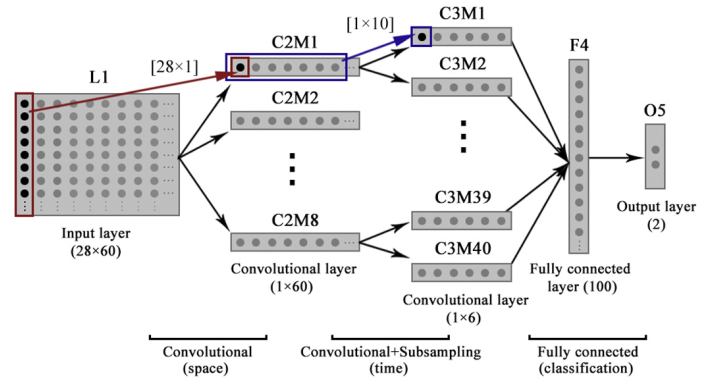
\includegraphics[height=0.6\textwidth]{images/2017_1trial_MIEEG_DNN_arch.png}
        \caption{CNN architecture proposed by \cite{2017_1trial_MIEEG_DNN}(source)}
        \label{fig:2017_1trial_MIEEG_DNN_arch}
    \end{figure}

\cite{2018_EEGNet} designed a single compact CNN architecture that can classify EEG signals from different paradigms using Depthwise and Separable CNNs. The raw EEG signal is convolved with a 1D convolutional filters with a filter length of half of the input sampling rate, resulting in feature maps containing band-passed EEG signal. The spatial information is obtained further using Depthwise convolution, the filters trained in this layer works as a spatial filter. This operation on band-passed EEG signal information enables extraction of frequency specific spatial filters. Finally Separable convolution is applied along with a Pointwise convolution to summarize individual feature maps and optimally combine them. The simple flow diagram given in the figure \ref{fig:eegnet_arch} shows how the depthwise separable convolutions are performed for classification. In this work, this architecture is chosen and implemented for its simplicity and adaptability to different EEG paradigms and experiments.

\begin{figure}[H] 
    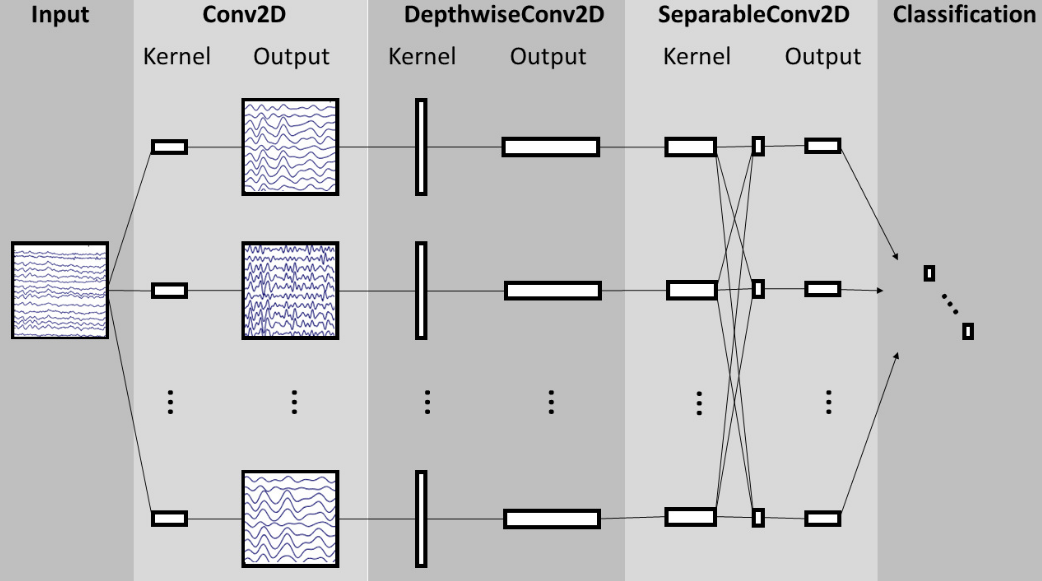
\includegraphics[height=0.6\textwidth]{images/eegnet_arch.png}
    \caption{EEGnet architecture. Source \cite{2018_EEGNet}}
    \label{fig:eegnet_arch}
\end{figure}

\section{Temporal Information}

Recurrent Neural Networks are vastly used in time series applications. They are inherently good at capturing dynamic information in serial data. RNNs have the problem of vanishing or exploding gradients which are overcome by replacing RNN nodes by LSTM cells. LSTM cells have a more complex internal structure that enables to remember data over a long or short time. A typical LSTM cell is shown in figure \ref{fig:lstm_cell}.

    \begin{figure}[H] 
        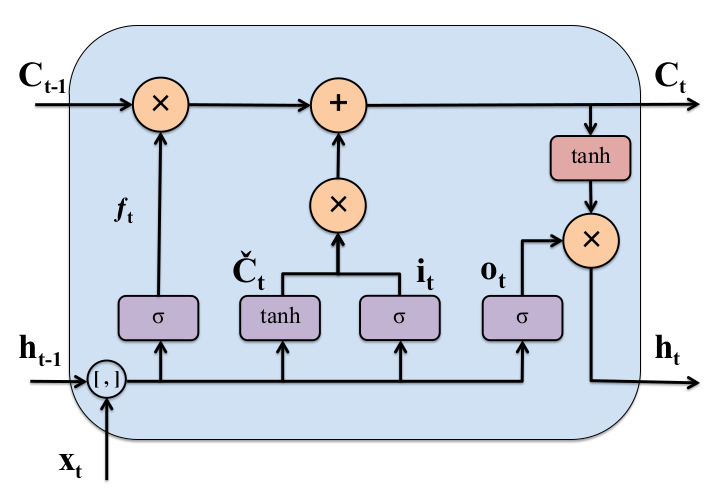
\includegraphics[height=0.6\textwidth]{images/lstm_cell.png}
        \caption{A LSTM cell structure. Source \cite{2018_DL_LSTM}}
        \label{fig:lstm_cell}
    \end{figure}
    
Attention mechanism is generally used at the end of an RNN model to find and weigh importance of each discriminative feature, that assures high classification scores. It is used in Natural Language Processing (NLP) \cite{2018_DL_LSTM} to find the contribution of each word to improve the scores. It amplifies the result by aggregating the hidden states and weighing their relative importance. 

\cite{2019_DLSTM_MI} proposed a solution for classification of hand movements from EEG using a deep attention-based LSTM network by first extracting time and frequency domain features from the EEG signals and passing them to the LSTM input layer. The attention layer captures the importance of the EEG information varying through time where discriminative information with higher importance is assigned higher scores, which results in higher classification results. Time and frequency domain features extracted are listed in \ref{fig:2019_DLSTM_MI_Table2}. The last hidden state of the LSTM is multiplied with trainable weights to capture more discriminative task related features which form the attention mechanism. The network uses 297 features from 7 time steps in each of the 2 second time segment. The entire architecture is given in the figure \ref{fig:2019_DLSTM_MI_arc}. This architecture has been implemented and studied in this thesis.

    \begin{figure}[H] 
    \begin{center}
        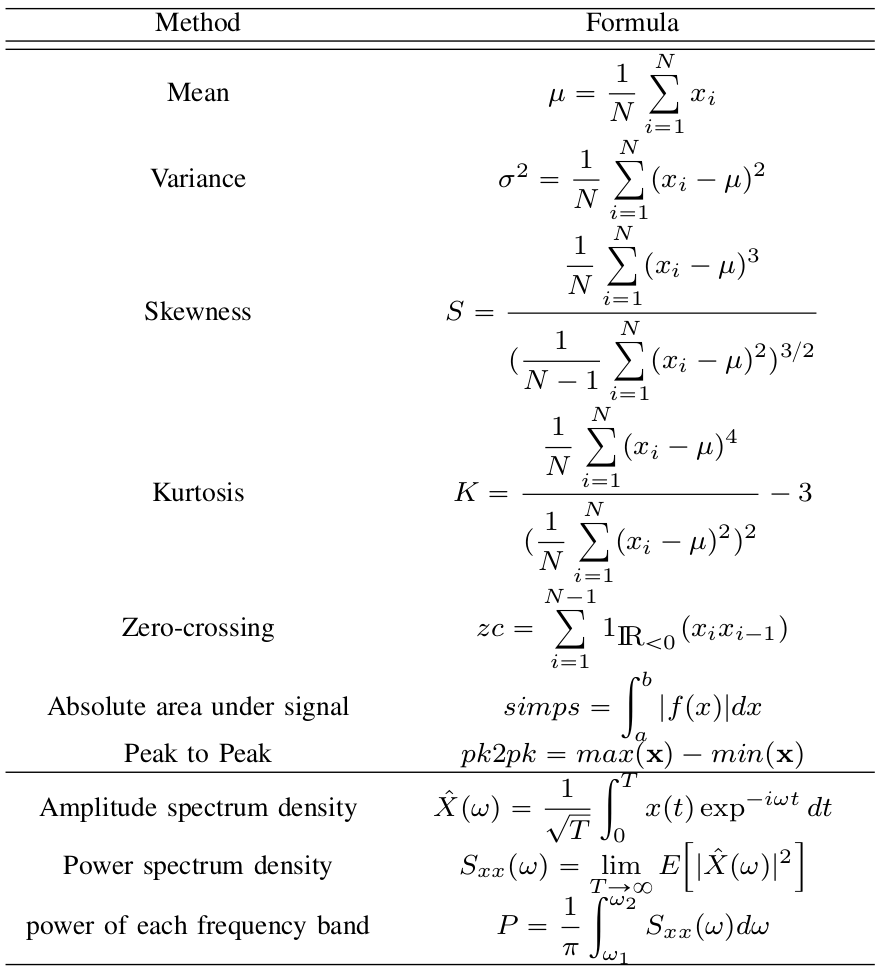
\includegraphics[height=0.6\textwidth]{images/2019_DLSTM_MI_Table2.png}
        \caption{The table of features used by \cite{2019_DLSTM_MI}(source)}
        \label{fig:2019_DLSTM_MI_Table2}
    \end{center}
    \end{figure}

    \begin{figure}[H] 
    \begin{center}
        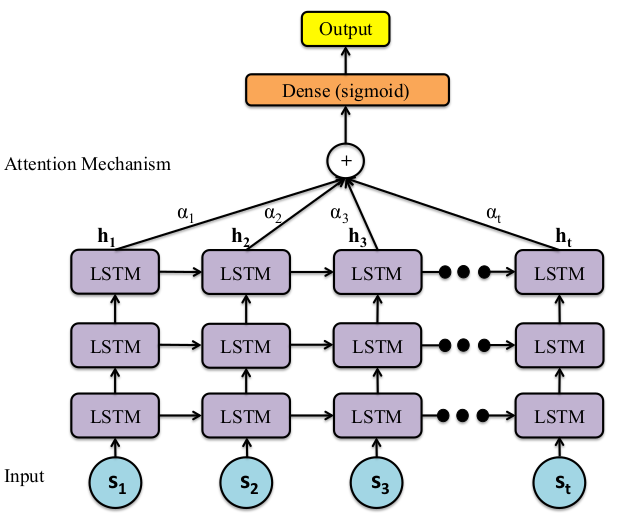
\includegraphics[height=0.6\textwidth]{images/2019_DLSTM_MI_arc.png}
        \caption{A LSTM based architecture proposed by \cite{2019_DLSTM_MI}(source)}
        \label{fig:2019_DLSTM_MI_arc}
    \end{center}    
    \end{figure}

\section{Spatio-Temporal Information}

\cite{2021_DL_LSTM_MI} introduced the cascade and parallel convolutional recurrent neural network to learn the spatio-temporal dynamics of EEG data. The method involves converting 1-dimensional EEG sequences to 2-dimensional EEG meshes, the values of the 2D meshes corresponds to the amplitude from each electrode. At time $t$, the 1D data from all the $n$ electrodes $$r = x_i,  \forall i \in n$$ is converted to 2D mesh with $n$ points and the vacant spaces are set to zero. The 2D meshes are created for each time instance $t$, stacked for a specific time interval $s$ and passed into a cascaded convolutional recurrent neural network \ref{fig:2021_DL_LSTM_MI_CCRNN}. 
    \begin{figure}[H] 
    \begin{center}
        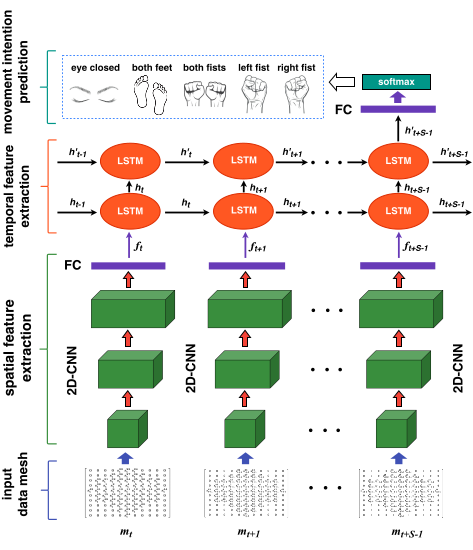
\includegraphics[height=1.0\textwidth]{images/2021_DL_LSTM_MI_CCRNN.png}
        \caption{A Cascaded convolutional recurrent neural network based architecture proposed by \cite{2021_DL_LSTM_MI}(source)}
        \label{fig:2021_DL_LSTM_MI_CCRNN}        
    \end{center}
    \end{figure}

The network first performs spatial feature extraction by a series of $s$ parallel convolution layers followed by a linear layer that fattens the information. The temporal features are extracted from the data by passing the flattened data to the LSTM layers and the output of the last LSTM cell is used to predict the movement intention using softmax as activation layer. \cite{2021_DL_LSTM_MI} also suggests using CNNs and RNNs separately and later concatenate the outputs of the last layers to predict the motor intention of the user using softmax activation layer.

\cite{2021_hDL_BCI} provides  systemic review of several Hybrid Deep Learning models used in BCI research. The study reveals that CNN-RNN hybrid deep learning architectures with Adam optimizer are the most widely researched for extracting spatial-temporal features from the EEG data and the average accuracy is 80 percentage across several datasets. 

\cite{2022_MI_DL_Multilevel} extracts domain-invariant multi-level spatial-temporal features to tackle domain differences. This is done by minimizing the source and target distribution distance.

While the above techniques proposed 2D convolutional neural networks, \cite{2020_DL_LSTM_EEG} proposed 1D CNN-LSTM architecture for automatic recognition of epileptic seizures through EEG signal analysis. Here the EEG data is preprocessed and normalized before the high level spatial information is extracted by the 1D-CNNs and the temporal features by the LSTM layer figure \ref{fig:2020_DL_LSTM_EEG_arch}.

    \begin{figure}[H] 
    \begin{center}
         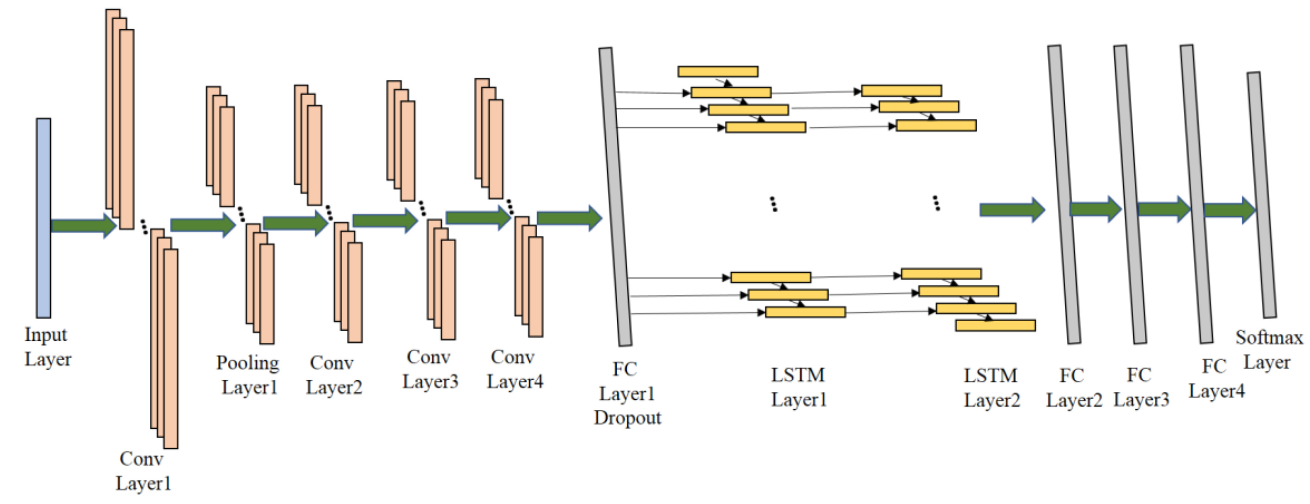
\includegraphics[width=1\textwidth]{images/2020_DL_LSTM_EEG_arch.png}
        \caption{A CNN-LSTM architecture proposed by \cite{2020_DL_LSTM_EEG}(source)}
        \label{fig:2020_DL_LSTM_EEG_arch}       
    \end{center}
    \end{figure}
    
\section{Summary}
Deep Learning is widely been used in BCI systems and researches. Several architectures are developed for a more specific task or problem in BCI. However only few architecture claim adaptability to different BCI applications. Many architectures are discussed above did not require manual removal of artifacts, as they were parameterized and learnt during the process of training. These systems however require retraining and calibration to work for different users and different hardware configurations. In the next chapter, all the implemented algorithms are compared using different datasets on various basis.

\chapter{Comparison and Benchmarking}
\section*{Introduction}

\section{Spatial Information}

\section{Temporal Information}

\section{Spatio-Temporal Information}

\section*{Summary}

% Conclusions / Findings
\chapter{Challenges and Conclusions}
\section*{Introduction}

\section{Challenges}

\section{Conclusion}

\section*{Summary}

% Reflective analysis
\chapter{Reflective Analysis}
\input{chapters/reflective-analysis.tex}





% end of thesis body
% --------------------------
% Print out the references
\printReferences
% Appendices: feel free to comment these out if you are 
% not going to use them.
%% Writing appendices is super super easy in LaTeX. You just write
% \appendix to demarcate where the normal content ends and the appendices start. After \appendix, chapters (started with \chapter) are considered as appendices.
%
% In this example though, we're using the appendices environment. Long story short, this is because we want some fancy titles in the toc.
\begin{appendices}

% Appendix A
% ----------

\chapter{Some random python code}
This template includes the \texttt{minted} package, which allows you to import code and syntax highlight it. For example, the text below is imported directly from the \texttt{code/test.py} file using the \textbackslash\texttt{inputminted} command:

\begin{framed}
    \inputminted{python3}{code/test.py}
\end{framed}

And here is a snippet of Python with the \texttt{minted} environment:

\begin{framed}
\begin{minted}[breaklines]{python}
# Why don't you try running this?
# See what it does? hm?

m = [ 2, 3, 0, 1, 4 ];
x = [ 'rmdq', 'd', 'n`slk', 'odftp`v)', 'hdk' ];

c = ''.join(list(map(lambda y: chr(ord(y) ^ 5).upper() + ' ' if y != ' ' else '  ', ' '.join([ x[m[i]] for i, v in enumerate(x) ]))));

print('%s\r\n%s\r\n%s\r\n' % ('=' * len(c), c, '=' * len(c)));
\end{minted}
\end{framed}

\cleardoublepage
Minted supports many, many languages -- so you're not just limited to Python. For example, here's some random C++ code.

\begin{framed}
\begin{minted}[breaklines]{cpp}
void CTimesTable::Print(const int number, const int upTo) const
{
    for(int i = 1; i <= upTo; i++)
        printf("%d x %d = %d\r\n", number, i, number * i);
}
\end{minted}
\end{framed}







% Appendix B
% ----------

\chapter{Some other stuff}
Here is just an example of some other stuff.

% End of appendices
\end{appendices}
\end{document}
